\section{Задание 2}

Создать HTML-страницу, которая при загрузке выводит в текстовое поле формы, сколько дней осталось до каникул.

\begin{center}
  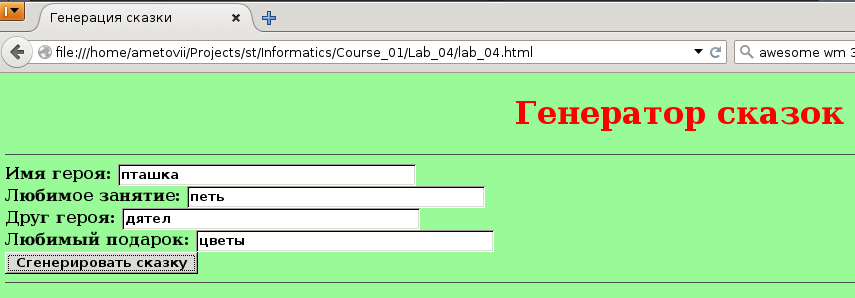
\includegraphics{img/Exercise_02/01.png}
\end{center}

Исходный код \verb|exercise_02.html|:

\begin{verbatim}
<!doctype html>
<html>
  <head>
    <title>Сколько дней до каникул?</title>
    <meta charset='utf-8' />
  </head>
  <body>
    До каникул осталось
    <input id='dayBeforeHoliday'></input>
    дней.
    <script>
      var todayDate=new Date();
      var holidayDate=new Date();
      holidayDate.setMonth(0);
      holidayDate.setDate(25);
      holidayDate.setFullYear(2016);
      var inputObject =
	  document.getElementById("dayBeforeHoliday");
      inputObject.value=(holidayDate-todayDate)/86400000;
    </script>
  </body>
</html>
\end{verbatim}
